\documentclass{llncs}

\usepackage{llncsdoc}
\usepackage{graphicx,url}
\usepackage[brazil]{babel}
\usepackage[utf8]{inputenc}
\usepackage{float}
\usepackage{setspace}

\usepackage{tabularx}
\usepackage{cite}
\usepackage{hyperref}
\usepackage{comment}
\usepackage{scalefnt}

\begin{document}
\sloppy
\title{Abordagem e plataforma para o monitoramento de métricas estáticas de código-fonte}

\author{Diego Camarinha\inst{1},Rafael Manzo\inst{1},Paulo Meirelles\inst{1}}

\institute{Instituto de Matemática e Estatística -- Universidade de São Paulo (USP)
  \email{\{diegoamc,manzo,paulormm\}@ime.usp.br}}

\maketitle

%------------------------------------------------------------------------------

\begin{abstract}

% Contexto
A facilidade de desenvolvimento e manutenção de um \textit{software} está
diretamente relacionada com a qualidade de seu código-fonte.
% Problema
No entanto, analisá-lo impõe dificuldades como, por exemplo, definir as
métricas e interpretar o resultado de uma medição. Além disso, essa prática
ainda não é comum em ambientes de desenvolvimento. Outro problema é a falta de
ferramentas livres que integrem coletores de métricas para diversas liguagens.
% Soluções propostas
Neste artigo, apresentamos uma abordagem para o monitoramento de métricas de
código-fonte, bem como uma plataforma \textit{web} livre para a avaliação
colaborativa de código-fonte, chamada Mezuro. Essa abordagem, apoiada pelo
Mezuro, fornece um meio para comparar projetos e compartilhar conhecimento
sobre métricas, ensinando a configurá-las e interpretá-las.

\textbf{Palavras-chave:} análise estática, métricas de código-fonte, software
livre.

\end{abstract}

%------------------------------------------------------------------------------

\section{Introdução}
\label{sec:intro}

Métricas estática de código-fonte são medidas extraídas a partir das análises
léxica e sintática deste sem compilá-lo ou executá-lo e podem ser primitivas ou
compostas, ou seja, formadas pela composição de uma ou mais métricas
primitivas. Sua principal função é fornecer informações sobre complexidade,
compreensão, testabilidade, manutenibilidade e evolução do
código~\cite{Henderson-Sellers96,Sato07}

Exemplos de métricas podem ser simples como linhas de código e quantidade de
métodos por classe ou complexas como conexões aferentes de uma classe. Hoje
existem diversas ferramentas para a extração de métricas como
pylint\footnote{\url{http://www.pylint.org/}} (Python),
metric\_fu\footnote{\url{https://github.com/metricfu/metric_fu}} (Ruby) e
Analizo\footnote{\url{http://www.analizo.org/}} (C/C++ e Java), cada uma com
diferentes graus de usabilidade, padrões e conjuntos de métricas, sendo
necessária a criação de uma plataforma que reúna, organize e apresente essas
informações para o usuário.

Por meio da avaliação de métricas de código-fonte podemos definir como está a
qualidade do \textit{software} e pensar em estratégias interessantes para lidar
com a chamada ``crise do \textit{software}'' \cite{naur1969software}. Esta
afirma que, com o crescimento da capacidade computacional, mais problemas
difíceis passam a ter solução viável, mas que, por outro lado, a complexidade
da interface para uso dos novos equipamentos (\textit{hardware}) e do processo
de desenvolvimento atuais combinados com a complexidade dos problemas exacerbam
falhas do \textit{software}. Assim, o controle da qualidade de um
\textit{software} durante sua evolução no tempo torna-se uma ferramenta para
identificar e prevenir tais falhas.

Entretanto, incorporar esta avaliação às metodologias de desenvolvimento de
\textit{software} não pode ser um processo manual em razão do risco desta
prática cair em desuso. Isto se deve ao fato de que as ferramentas de extração
de métricas, em geral, não apresentam uma interface amigável para seres humanos
lerem seus resultados e muito menos um padrão entre si. 
%
Além disso, não existe um consenso sobre qual conjunto de métricas é relevante para
se avaliar a qualidade do código e uma abordagem de análise estatística para indicar
valores bons ou ruins de tais métricas\cite{meirelles2013monitoramento}.

Entre nossos estudos, avaliamos a distribuição e correlações dos valores das
métricas de 38 projetos de software livre, dentre os com mais contribuidores
ativos em seus repositórios. Para tal, coletamos e analisamos os valores para
cada métrica em mais de 344.872 classes e módulos dos projetos
avaliados\cite{meirelles2013monitoramento}.
%
A partir dessas análises, definimos uma abordagem que permita a definição de
parâmetros, viabilizando estudos estatísticos que nos aproximem de uma
conclusão sobre os resultados das métricas coletadas.
%
Do ponto de vista prático, desenvolvemos um conjunto de ferramentas,
representada pela plataforma Mezuro, para a automação da avaliação de projetos
de software, com ênfase nos estudos e na seleção de métricas, o que
permite a análise de código-fonte ao longo do tempo.

%TODO: se couber, o que vem a seguir no artigo

%------------------------------------------------------------------------------

\section{Trabalhos relacionados}

Alguns estudos baseado em análise de métricas de código-fonte têm uma limitação
ao não avaliarem se a média das valores é uma medida representativa, ou seja,
informativa estatisticamente, para tais
análises\cite{meirelles2013monitoramento}.
%
Mesmo estudo mais recentes, baseados nas análises de métricas também não deixam
claro a representatividade da média das métricas. Por exemplo, Williams at
at.\cite{williams2010} determinaram os tipos de mudanças na arquitetura de
software e propuseram uma caracterização dessas mudanças, o que também envolveu
a análise de métricas de complexidade de código-fonte.
%
Terceiro e seu grupo~\cite{terceiro2009, terceiro2012:csmr, terceiro2010:dcoss,
terceiro2010:core-periphery} realizaram estudos para definir uma caracterização
da complexidade estrutural em sistemas de software livre.
%
Eles analisaram a complexidade estrutural média entre todos os módulos de 13
projetos de software livre, de diferentes domínios de aplicação e linguagens de
programação, observando o histórico de mudanças desses sistemas, porém,
limitados ao considerar a média representativa para suas análises.
%

Entretanto, alguns outros trabalhos relacionados mencionam que métricas de
software, incluindo as métricas de código-fonte, têm sido analisados como dados
que são leis de potência~\cite{clauset2007}, em especial as métricas de
orientação a objetos.
%
Isso significa que, de acordo com esses trabalhos, as métricas de código-fonte
possuem distribuições estatísticas que têm como característica geral ter cauda
longa e ser de escala livre, o que significa que a média não é um valor
informativo~\cite{clauset2007}.

Entretanto, observarmos que a maioria desses trabalhos estavam analisando
apenas códigos em Java e generalizando suas observações para todos os projetos
orientados a objetos.
%
Além disso, os critérios de seleção dos projetos avaliados não contemplam, em
uma amostra maior, os principais projetos de software livre disponibilizados,
em particular os com mais desenvolvedores ativos e atualizações nos repositório
(atividade de desenvolvimento).

Por exemplo, Wheewldon et al.\cite{Wheeldon2003} avaliaram 4 projetos em Java:
JDK (Java Development Kit), Apache, Ant e Tomcat.
%
Eles identificaram leis de potência para as métricas de número de atributos,
número de métodos. Um estudo com poucos projetos e poucas métricas, mas que
levantou a questão das leis de potências.
%
Potanin et al.\cite{Potanin2005} analisaram 35 programas Java e observaram que,
neles, os relacionamentos entre os objetos constituem um grafo livre de escala,
que difere de um grafo com arestas distribuídas aleatoriamente. Em um de grafo
livre de escala, uma vez que a distribuição dos graus de seus vértices seguem
uma lei de potência, a média não é representativa. Fizeram constatações
interessantes, mas limitados a Java e a seleção não clara dos projetos não
permite generalizar os resultados.
%
Baxter et al.\cite{Baxter2006} coletaram métricas de 56 projetos de software
livre em Java.  Eles demonstram que nem todas as métricas estão sob leis de
potência, indicando que algumas métricas, como grau de entrada
(\textit{fan-in}) e número de subclasses, seguem leis de potência, mas outras
métricas não, como grau de saída (\textit{fan-out}), número de atributos e
número de atributos públicos.
%
Louridas et al.\cite{Louridas2008} avaliaram partes de 11 projetos (10 livres e
um restrito) escritos em Java, C, Ruby e Perl.
%
Eles investigaram apenas o grau de entrada (\textit{fan-in}) e de saída
(\textit{fan-out}) dos módulos e classes. Seus resultados  indicam que essas
métricas possuem distribuições na família de leis de potência, independente do
paradigma de programação.
%
Em relação à métrica de grau de saída, o estudo de Baxter et
al.\cite{Baxter2006} apresenta resultados diferentes. Isso nos levou a refletir
pela literatura que as métricas que trabalhamos nesta tese não são governadas
necessariamente pelas leis de potência; além disso, não podemos generalizar
para uma distribuição normal.

Mesmo com esses estudos sobre as leis de potência, observamos que, na área de
avaliação de métricas de código-fonte e visualização de software, os trabalhos
de Michele Lanza, em particular o seu livro \cite{Lanza2006}, são os mais
reconhecidos.
%
Entretanto, não se verifica cuidadosamente como seus dados foram analisados.
%
Lanza e Marinescu\cite{Lanza2006} definiram valores referência para 3 métricas
de código-fonte (número de métodos por classe, número de linhas de código
linhas de código e complexidade ciclomática por método) baseado em informações
estatísticas.
%
Eles avaliaram essas 3 métricas em 37 programas desenvolvidos em C++ e 45 em
Java, entre projetos de software livre e software restrito.
%
Lanza e Marinescu\cite{Lanza2006} generalizaram as análises e consideraram os
valores das métricas como uma distribuição Normal.
%
Dessa forma, um cálculo simples com a média e o desvio padrão foi feito para
definir o que eles denominaram de intervalos de referência:
%
o valor de uma métrica é considerando fora desse padrão quando ele é 50\% maior
que o valor do intervalo determinado. Em resumo, eles assumem a média como um
valor informativo para suas análises.

Na mesma linha do trabalho de Lanza e Marinescu\cite{Lanza2006}, na tentativa
de definir valores de referência, Ferreira et al.\cite{Ferreira2009} conduziram
um estudo que analisou diferentes métricas para 40 programas, de 11 diferentes
domínios de aplicação, desenvolvidos em Java.
%
Esse trabalho sugere intervalos qualitativos para 6 métricas: COF
(conectividade), LCOM (coesão), DIT (profundidade da arvore de herança), ACC
(conexões aferentes), NPA (atributos públicos) e NPM (número de métodos
públicos).
%
Eles argumentam que essas métricas podem ser modeladas pelas distribuições
Weibull e Poisson, que são leis de potência, sendo possível identificar valores
típicos para tais métricas e usá-los com referência para o desenvolvimento de
software de qualidade.
%
Mesmo sendo uma tentativa de definir valores de referência, a limitação pela
linguagem Java e por não contemplar os principais projetos de software livre,
somado às contradições e generalização dos trabalhos relacionados citados, nos
levou a verificar em detalhes as distribuições de cada métrica.
%
Por fim, em particular, na abordagem de \cite{Ferreira2009} não ficou clara a
definição dos pontos de corte para a indicação dos intervalos, bem como nos
testes das distribuições foi usada uma ferramenta restrita (fechada), o que
impede a reprodução na íntegra do referido
estudo\cite{meirelles2013monitoramento}.

%% trabalhos que questionam a generalização e exclusivadade da power law

Nesse contexto, como visto, as distribuições estatísticas de métricas de
código-fonte têm sido estudadas.
%
Por um lado, em particular as métricas para códigos escritos em linguagens
orientadas a objetos, no caso Java, parecem obedecer a leis de
potência~\cite{Wheeldon2003, Potanin2005, Concas2007, Ferreira2009, Yao2009}.
%
Por outro lado, observamos que há indícios que não necessariamente algumas
métricas têm suas distribuições de modo que seu comportamento siga uma lei de
potência~\cite{Baxter2006, Lanza2006, Herraiz2011, Herraiz2012}.

Estamos argumentando e apresentando aqui que não há consenso sobre se as
métricas de código-fonte podem ser melhor descritas usando leis de potência,
distribuição normal ou lognormal~\cite{meirelles2013monitoramento}.
%
Essa informação é relevante para determinarmos qual medida estatística (média,
mediana ou algum percentil) devemos observar para monitorarmos as métricas de
código-fonte.
%
Também, se há essa dispersão de abordagens sobre as distribuições das métricas
em códigos escritos no paradigma de orientação a objetos, que vem sendo o alvo
de estudos da maioria dos trabalhos, no contexto de projetos de software livre,
em que boa parte dos projetos são escritos em C\cite{robles2006:mining-large},
essa questão se apresenta mais aberta ainda.

%------------------------------------------------------------------------------

\section{Abordagem de monitoramento de métricas de código}
\label{sec:abordagem}

Ao constatarmos a contradição nos trabalhos da área em relação às distribuições
das métricas e observarmos o número limitado de métricas estudadas, geralmente
apenas em projetos escrito em Java, conduzimos estudos selecionando um conjunto
de 38 projetos de software livre (18 escritos predominantemente em C, 6 em C++
e 14 em Java), por exemplo, Linux Kernel, FreeBSD, Chrome, Firefox, Eclipse IDE
e Open JDK8, num total de 344.872 classes e
módulos~\cite{meirelles2013monitoramento}.

As métricas coletadas e analisadas para este estudo foram:
(ACC) Conexões aferentes de uma classe;
(ACCM) Média da Complexidade Ciclomática por método;
(AMLOC) Média do número de linhas de código por método;
(ANPM) Média do Número de Parâmetros por Método;
(CBO)Acoplamento entre objetos;
(DIT) Profundidade da árvore de herança;
(LCOM) Ausência de coesão em métodos;
(LOC) Número de linhas de código;
(NOA) Número de atributos;
(NOC) Número de filhos;
(NOM) Número de métodos;
(NPA) Número de atributos públicos;
(NPM) Número de métodos públicos;
(RFC) Respostas para uma classe;
(SC) Complexidade estrutural~\cite{meirelles2013monitoramento}.
%
Fizemos análises estatísticas detalhadas, desde a análise descritiva dos dados,
passando pela verificação do tipo de distribuição em cada métrica, até
chegarmos nos percentis dos valores das métricas das classes (ou módulos) de
cada um dos projetos.
%
Em resumo, nossos dados sinalizam que o monitoramento dessas métricas pode
variar de acordo com a linguagem de programação, domínio de aplicação ou mesmo
de acordo com a maturidade do projeto~\cite{meirelles2013monitoramento}.

%ACC
Por exemplo, no caso da métrica ACC, por conta da distribuição de Pareto
observada, sugerimos como referência de valores frequentes, os dados do
percentil 75, de forma que para projetos escritos em C, o código do Linux
sinaliza ter valores frequentes não tão bons quanto o do Android, mas factíveis
de serem usados como uma referência para C: de 0 a 2,0: muito frequente; de 2,1
a 7,0: frequente; de 7,1 a 13,0: pouco frequente; acima de 13,0: não frequente.
%
Para C++, o código do Firefox, mesmo com ACC não tão bom quanto o OpenOffice,
indica um equilíbrio para usarmos seus valores frequentes: de 0 a 2,0: muito
frequente; de 2,1 a 7,0: frequente; de 7,1 a 15,0: pouco frequente; acima de
15,0: não frequente.
%
Para Java, o Open JDK8 pode ser nossa referência ao observarmos os 14 projetos:
de 0 a 1,0: muito frequente; 1,1 a 5,0: frequente; de 5,1 12,0: pouco
frequente; acima de 12,0: não frequente.

%ACCM
Outro exemplo é que o tipo de distribuição para a métrica de complexidade
ciclomática (ACCM) varia entre os projetos.
%
Além da Weibull, dependendo do projeto, ela se ajusta ao \textit{Skew
Exponential Power}, que também vamos considerar como uma lei de potência, uma
vez que as distribuições que seguem as leis de potência são consideradas um
caso particular das distribuições Skew~\cite{Mahnke2012}.
%
Também, há casos em que a métrica ACCM se ajusta com a Sin-Arcsinh, que é um
caso especial das distribuições Beta, e assim também entendemos que a média não
é informativa para ela~\cite{jones2005}.

Da mesma forma, como apresentado para a métrica ACC, no caso da ACCM,
observamos o percentil 75 dos dados das métricas, e não a média, para podermos
sugerir seus valores como frequentes.
%
Para C, de 0 a 3,6 muito frequente; de 3,1 a 5,3 frequente; de 5,4 a 7,0 pouco
frequente, acima de 7,0 não frequente.  Para projetos escritos em C++, de 0 a
2,0 muito frequente; de 2,1 a 4,0 frequente; 4,1 a 6,0 pouco frequente; acima
de 6 não frequente.
%
Para os projetos Java, de 0 a 2,8 muito frequente; de 2,9 a 4,4 frequente; de
4,5 a 6,0 pouco frequente; acima de 6 não frequente.

%AMLOC
Também para a métrica AMLOC há uma variação entre os tipos de distribuição.
Além da Pareto tipo 2, entre os projetos, a AMLOC ajusta-se com a \textit{Skew
Exponential Power} e \textit{Skew t}, que seguem as leis de potência, como
argumentamos para a métrica ACCM, bem como a Sin-Arcsinh.
%
Entretanto, há projeto em que a distribuição da métricas AMLOC se ajusta com
\textit{Generalized t}, \textit{Box-Cox Power Exponential} e \textit{Box-Cox
t}.
%
A Generalized t (ou Student's t ou simplesmente distribuição t) tem a média
como um valor informativo, uma vez que estima a média de uma população
distribuída normalmente.
%
As distribuições da família de Box-Cox são conhecidas como uma distribuição de
potência normal e são muitas vezes modelas como normal em alguns
estudos~\cite{Rigby2006}.
%
Com isso, nesses casos, a média é uma médida informativa. Isso também pode
sinalizar que, dependo do conjunto de projetos, a abordagem apresentada por
Lanza e Marinescu~\cite{Lanza2006}.
%
Assim, também nos faz considerar a mediana como um dado informativo para o
número médio de linhas de código por métodos.

Uma vez considerando a mediana um valor representativo, nossa interpretação
para os valores frequentes da métrica AMLOC tem como primeiro ponto de corte o
percentil 50.
%
Mais uma vez, vamos sinalizar os valores de AMLOC para o Linux, Firefox e Open
JDK8 como os mais equilibrados.
%
Na busca de uma melhor referência, por exemplo, para os códigos em C, os
valores do código do GCC para a métrica AMLOC se apresentam mais indicados.
%
Em nossa abordagem, estamos indicando esses três projetos como referência entre
os de suas linguagens.
%
Portanto, estamos sugerindo que esses nossos dados tenham outras
interpretações, por outros pesquisadores, e que possam gerar outros valores
frequentes de referência, de acordo das diferentes interpretações.
%
Nosso objetivo não é definir valores frequentes em si, mas mostrar como é
possível achá-los e indicá-los: uma maneira é interpretar esse nosso conjunto
de dados ou reproduzir nossas coletas em outro projetos para indicar os valores
frequentes também baseado neles, preferencialmente somando-se aos avaliados
aqui neste trabalho.

Baseado nos valores observados no código do Linux, para um código escrito em C:
de 0 a 15,6 muito frequente; de 15,7 a 25,5 frequente; de 25,6 a 39,3 pouco
frequente; acima de 39,3 não frequente.
%
Para os projetos em C++, de acordo com valores do Firefox: de 0 a 8,0 muito
frequente; de 9 a 19,5 frequente; 19,6 a 37 pouco frequente; acima de 37 não
frequente.
%
Por fim, para os projetos escritos em Java, conforme observado no código do
Open JDK8, temos para a AMLOC: de 0 a 8,3 muito frequente; de 8,4 a 18
frequente; de 19 a 34 pouco frequente; acima de 34 não frequente.

O estudo completo, contemplando as demais métricas, é discutido por Meirelles,
em sua tese de doutorado~\cite{meirelles2013monitoramento}. Com os exemplos
apresentados, a abordagem proposta é o acompanhamento de métricas de
código-fonte, flexibilizando a análise, ou seja, dependendo do projeto, da
linguagem e até do tipo de métricas em questão.
%
Em muitos casos, o indicado é saber comparar o projeto com ele mesmo ao longo
do tempo. Para isso, a abordagem de análise estatística, observando a
distribuição e identificando o melhor ponto (percentil) de análise se faz
necessário; ao contrário de usar como parâmetro referências genéricas.
Entendendo a complexidade dessa abordagem na prática, uma forma de
concretizá-la, foi desenvolver uma plataforma que permitisse tal flexibilização
por projeto analisado e ao mesmo tempo pudesse ser compartilhado em rede para
outros, se for do mesmo escopo e contexto, por exemplo.

%------------------------------------------------------------------------------

\section{Plataforma de monitoramento de métricas de código}
\label{sec:mezuro}

Para aplicação da abordagem discutida neste artigo, uma ferramenta com as
seguintes características se faz necessária, para a introdução deste tipo de
avaliação constante às metodologias de desenvolvimento de software: (i)
interface que agrupe as diversas ferramentas disponíveis; (ii) permita seleção
e composição de métricas de forma flexível; (iii) manutenção de um histórico de
evolução; (iv) exiba os resultados de forma amigável.

Em 2009, iniciamos a concepção de uma plataforma de monitoramento de métricas
de código-fonte denominada Mezuro\cite{mezuro2012}, disponível em
{\url{http://mezuro.org}}.
%
Em uma visão geral, o Mezuro é dividido em duas partes: processamento e cálculo
de métricas de código-fonte (Kalibro, um \textit{webservice}); e a interface
gráfica para apresentação dos resultados (Prezento, uma aplicação
\textit{Web}).

O Prezento é a nova versão da camada de visualização do Mezuro, que começou a
ser reescrito, em 2013, principalmente com o intuito de trazer ao projeto tudo
o que as tecnologias mais recentes têm a oferecer, mas também eliminar
funcionalidades não essenciais em suas versões iniciais. Assim, o Prezento foi
escrito em \textit{Ruby}, utilizando o arcabouço \textit{Ruby on Rails}
%
No processo de evolução do Mezuro, uma parte considerável do código legado foi
empacotada em uma gema Ruby, denominada \textit{kalibro\_gem}, a licença
\textit{Affero General Public License} versão 3 (AGPLv3) foi adotada e uma
interface completamente redesenhada foi desenvolvida, ou seja, o Prezento.
%
Nessa interface, o usuário é o responsável por definir o conjunto de métricas a
ser utilizado para realizar cálculos, com a possibilidade de armazenar os
resultados para comparações futuras. Seu objetivo é (i) aproximar-se de um
consenso acerca de quais métricas devem ser empregadas na análise da qualidade
de um código-fonte; e (ii) buscar os valores dessas métricas que definem a
qualidade de um código-fonte.

O Kalibro\cite{de2013kalibro} foi inicialmente escrito em Java, mas também no
processo de evolução do projeto Mezuro, a partir de 2014, passou a ser
reescrito em Ruby, com o objetivo de unificar as tecnologias do projeto e
corrigir os problemas da versão original em Java.
%
Isso porque, os resultados dos testes de escalabilidade indicaram que o módulo
da plataforma que mais exigia capacidade de processamento era o que calculava e
analisava métricas de repositórios, ou seja, o Kalibro.
%
Para melhor definir a nova arquitetura do Kalibro, monitoramos seus parâmetros
de escalabilidade utilizando o arcabouço \textit{Scalability Explorer}
\cite{moura2013automated} para gerenciar a carga de requisições e a frequência
com que elas eram enviadas. 
%
Em suma, dependendo do número de requisições recebidas e do número de núcleos
que o servidor possuía, o Kalibro original entrava em estado de impasse. Além
disso, a arquitetura original era monolítica, ou seja, uma mudança em um ponto
do código culminava na obrigação de mudar outros diversos pontos do código.
%
As vantagens decorrentes da reescrita do Kalibro foram prover a maior
modularidade do sistema (ou seja, dos serviços), e, por ser software livre,
facilitar o entendimento do código para novos contribuidores.

%------------------------------------------------------------------------------

\subsection{Arquitetura do Mezuro}
\label{sec:arquitetura}

  Desde a sua primeira implementação até a sua reescrita completa, a arquitetura do sistema evoluiu consideravelmente. Quando o projeto era integrado com o Noosfero, nosso sistema ficava preso às limitações tanto da tecnologia utilizada, que tinha que ser compatível com a do Noosfero, quanto da arquitetura de \textit{plugins}, que restringia nossa liberdade para expandirmos nossas funcionalidades.

  Após desacoplarmos o Mezuro do Noosfero, passamos a ter completa autonomia para usar as tecnologias que julgávamos ser mais adequadas para solucionar nossos problemas. Preocupamo-nos também em mantê-las atualizadas para termos as funcionalidades mais novas e as correções de defeitos antigos. Outra mudança importante foi a adoção do estilo arquitetural de micro serviços \cite{namiot2014micro}. A \textbf{figura \ref{fig:architecture-1}} ilustra a arquitetura do sistema, ao fim da reescrita da interface gráfica, por meio de um diagrama UML de sequência. A ilustração se refere ao processo de criação de uma configuração até os resultados finais de uma análise.

  \begin{figure}[H]
    \centering
    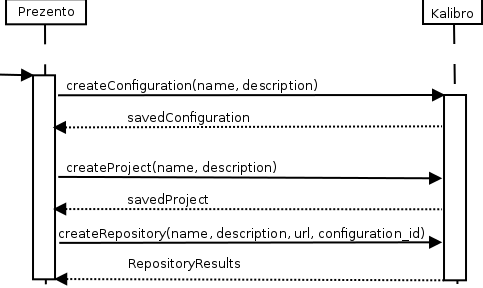
\includegraphics[width=\textwidth]{images/prev_processing_seq_diag.png}
    \caption{Arquitetura do sistema ao fim da reescrita da interface gráfica.}
    \label{fig:architecture-1}
  \end{figure}

  Com o projeto inteiramente reescrito, evoluímos a arquitetura para o estado atual (\textbf{figura \ref{fig:architecture-2}}) que representa as mesmas operações da figura anterior.

  \begin{figure}[H]
    \centering
      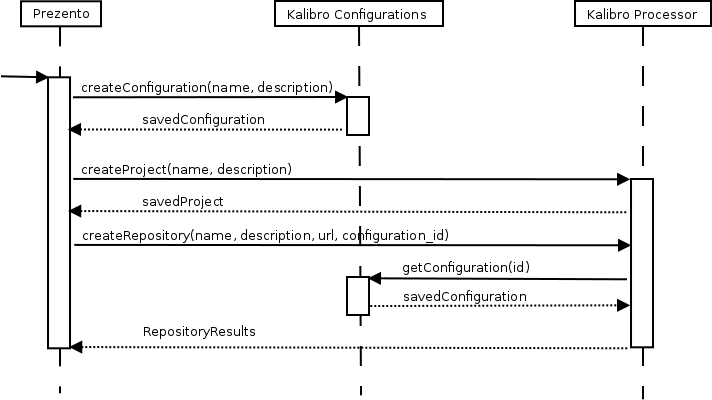
\includegraphics[width=\textwidth]{images/processing_seq_diag.png}
    \caption{Arquitetura do sistema ao fim da reestruturação do Kalibro.}
    \label{fig:architecture-2}
  \end{figure}

  Explorando mais a fundo a \textbf{figura \ref{fig:architecture-2}}, notamos que houve uma separação do serviço monolítico em dois serviços menores e especializados: o Kalibro Processor e o Kalibro Configurations. Essa mudança produziu mais complexidade do ponto de vista de quantidade de mensagens trocadas, o que pode causar a impressão de que a manutenabilidade do projeto piorou. Entretanto, com uma interface de comunicação bem definida, o aumento na troca de mensagens gera impactos mínimos que são compensados pela modularização e maior especialização dos serviços.

\section{Diferenciais} \label{subsec:motivacao}
As principais motivações para o surgimento de uma ferramenta como o Mezuro são os seguintes problemas:
\begin{itemize}
    \item Não há parâmetros de comparação consolidados entre projetos;
    \item Existem estudos, mas poucos dados empíricos;
    \item Ainda é dada pouca importância ao monitoramento de código.
\end{itemize}

\section{Por que usar o Mezuro?} \label{sec:projeto-mezuro}
Idealizado como uma plataforma de métricas de código, um dos diferenciais do Mezuro reside na possibilidade de gerar informação sobre o código-fonte de forma contínua: o usuário decide quando analisar novamente o projeto e acompanha detalhadamente a evolução das notas ao longo do tempo. Os resultados de cada análise são públicos, o que permite uma maior transparência entre o desenvolvedor e a comunidade que utiliza aquele \textit{software}. Assim, ela pode decidir se aquela solução atende ou não às suas necessidades e se deve depositar confiança na qualidade do \textit{software} desenvolvido.

\section{Principais funcionalidades}\label{sec:princ-funcionalidades}
No Mezuro, as funcionalidades podem ser divididas em dois grupos:
\begin{itemize}
  \item Projeto
    \begin{itemize}
    \item \textit{Download} do código-fonte a partir de repositórios (Git, Subversion, Bazaar etc) ou via arquivo compactado;
        \item Escolha da periodicidade do processamento do código (1 dia, 2 dias, semanal, quinzenal e mensal);
        \item Escolha de qual configuração de métricas cada repositório irá utilizar;
        \item Nota de cada métrica da configuração para cada arquivo do repositório;
        \item Análise gráfica de cada arquivo do repositório por meio de um gráfico de pontos com notas ao longo do tempo;
        \item Resultados públicos e acessíveis à comunidade.
    \end{itemize}
    \item Configuração
    \begin{itemize}
    \item Criação de configuração e a possibilidade de clonagem;
        \item Estatísticas sobre as configurações mais populares dentro da comunidade;
        \item Criação de intervalos qualitativos associados aos valores das métricas;
        \item Criação de grupos de leitura para a interpretação textual dos resultados das métricas;
        \item Combinações de métricas nativas para criação de análises compostas e mais complexas.
    \end{itemize}
\end{itemize}

\section{A rede social}\label{sec:user-potencial}
O Mezuro tem o formato de uma rede social, no qual os participantes podem ver a produção de terceiros por meio da avaliação dos projetos ou do clone das configurações. Essa interação mútua e aberta pode ser interessante para desenvolvedores, gerentes de projeto, auditores de \textit{software} e até mesmo uma equipe de desenvolvimento inteira. O objetivo final é criar uma comunidade que veja o valor de tais metodologias e como isso pode contribuir para o sucesso do seu projeto.

\section{Casos de uso}
Apresentaremos a seguir as duas principais funcionalidades da ferramenta ilustradas por meio de capturas de telas. Em todas elas, utilizamos uma conta já cadastrada no sistema (único privilégio necessário para realizá-las).

  \subsection{Criação de configuração}
  \begin{figure}[H]
    \centering
    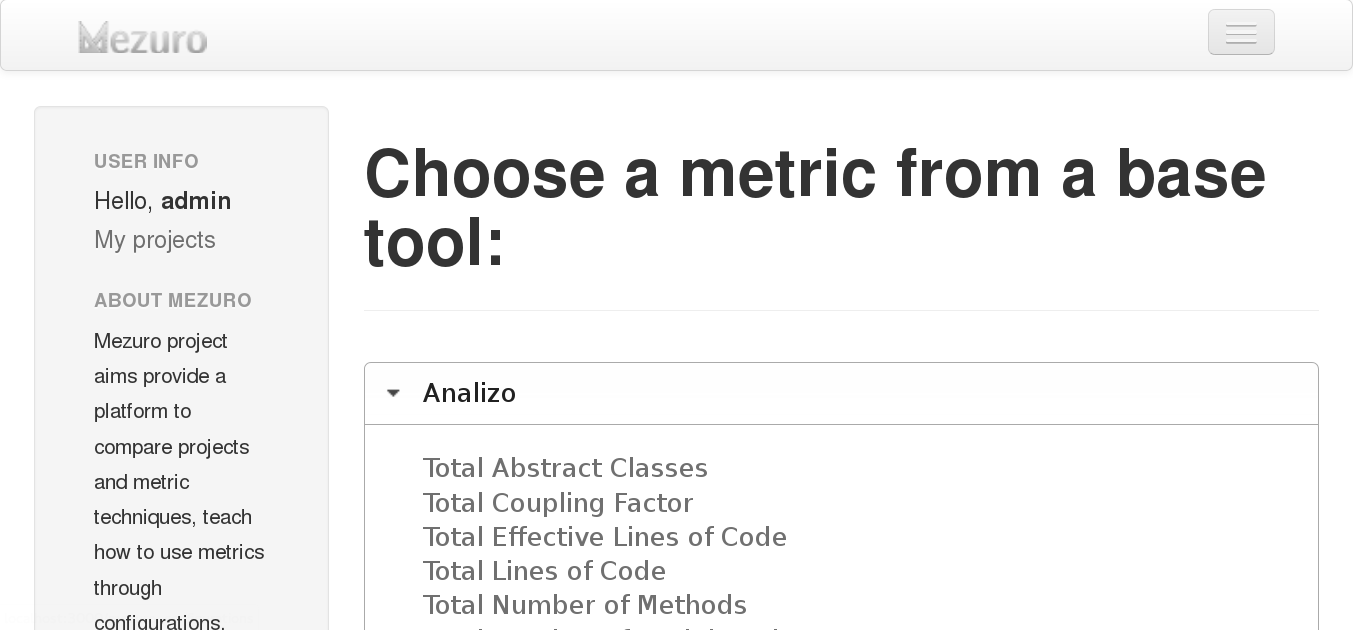
\includegraphics[width=\textwidth]{images/choose-metric.png}
    \caption{Interface para escolha de ferramenta extratora de métrica e escolha de uma métrica nativa para adicionar a uma configuração.}
    \label{fig:choose-metric}
  \end{figure}

  Criar uma configuração envolve 5 telas do sistema em 4 passos básicos:
  \begin{enumerate}
    \item Acessar a página de listagem de configurações;
    \item Clicando em ``New configuration'', preencher o formulário de criação de configuração e salvá-lo;
    \item Clicando em ``Add metric'', escolher a ferramenta de extração e qual métrica a ser usada (figura \ref{fig:choose-metric});
    \item Preencher o formulário (detalhado a seguir) e salvá-lo.
  \end{enumerate}

  Os passos 3 e 4 devem ser repetidos para cada métrica adicionada à configuração. O formulário de métrica (passo 4) é complexo se comparado ao de configuração mas, assim como os demais, cada campo possui detalhes sobre sua utilização. Aqui, destacamos os menos evidentes:
  \begin{itemize}
    \item \textbf{Aggregation Form:} Maneira com a qual o resultado de uma métrica será agregado (média, mediana, máximo, etc);
    \item \textbf{Reading Group:} Conjunto de intervalos usado para dar significado prático ao resultado calculado.
  \end{itemize}

  \subsection{Criação de projeto e avaliação de repositório}
  Criar um projeto envolve 2 passos básicos:
  \begin{enumerate}
    \item Acessar a página de listagem de projetos;
    \item Clicando em ``New project'', escolher o nome, a descrição e salvá-lo.
  \end{enumerate}

  \begin{figure}[H]
    \centering
    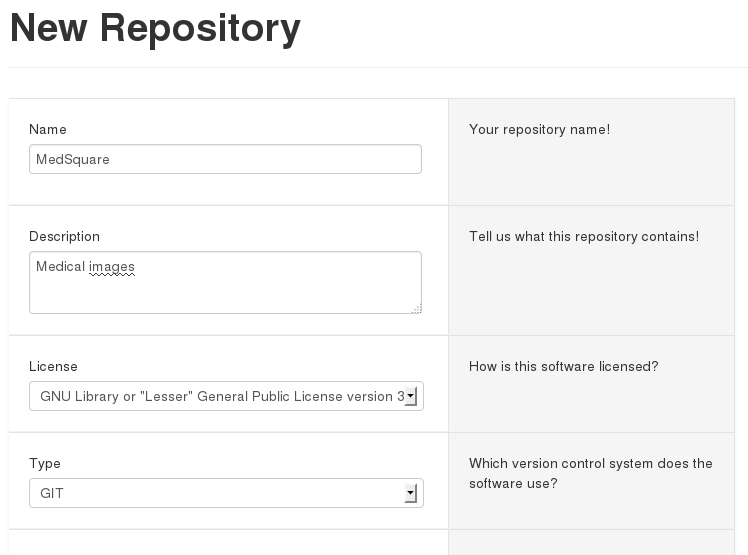
\includegraphics[width=\textwidth]{images/new-repository.png}
    \caption{Interface para criação de um novo repositório.}
    \label{fig:new-repository}
  \end{figure}

  Ao clicar em ``New repository'' entramos na criação do repositório a ser avaliado (figura \ref{fig:new-repository}). Alguns campos merecem destaque:
  \begin{itemize}
    \item\textbf{Type:} Tipo do repositório (também pode ser um zip ou tarball) onde o código está hospedado;
    \item\textbf{Address:} Endereço do repositório remoto ou o caminho absoluto no sistema de arquivos;
    \item\textbf{Process Period:} Periodicidade com a qual o código deve ser analizado pela ferramenta (diariamente, semanalmente etc);
    \item\textbf{Configuration:} Configuração de métricas que o usuário deseja utilizar para medir o código (pode ser escolhida dentre todas as configurações criadas pelos usuários).
  \end{itemize}
  Após preencher todos os campos e salvar o repositório, seu primeiro processamento será automaticamente ativado e o usuário será redirecionado para a página que exibe os resultados. Nela, ele poderá conferir dados do processamento (tempo gasto para o término de cada uma de suas fases) e navegar na árvore de módulos gerada, para que possa visualizar a nota, os resultados das métricas e suas interpretações para cada um deles (figura \ref{fig:results}). Além disso, ao clicar no nome de uma métrica calculada, um gráfico que representa a evolução dos seus valores ao longo do tempo será exibido.

  \begin{figure}[H]
    \centering
    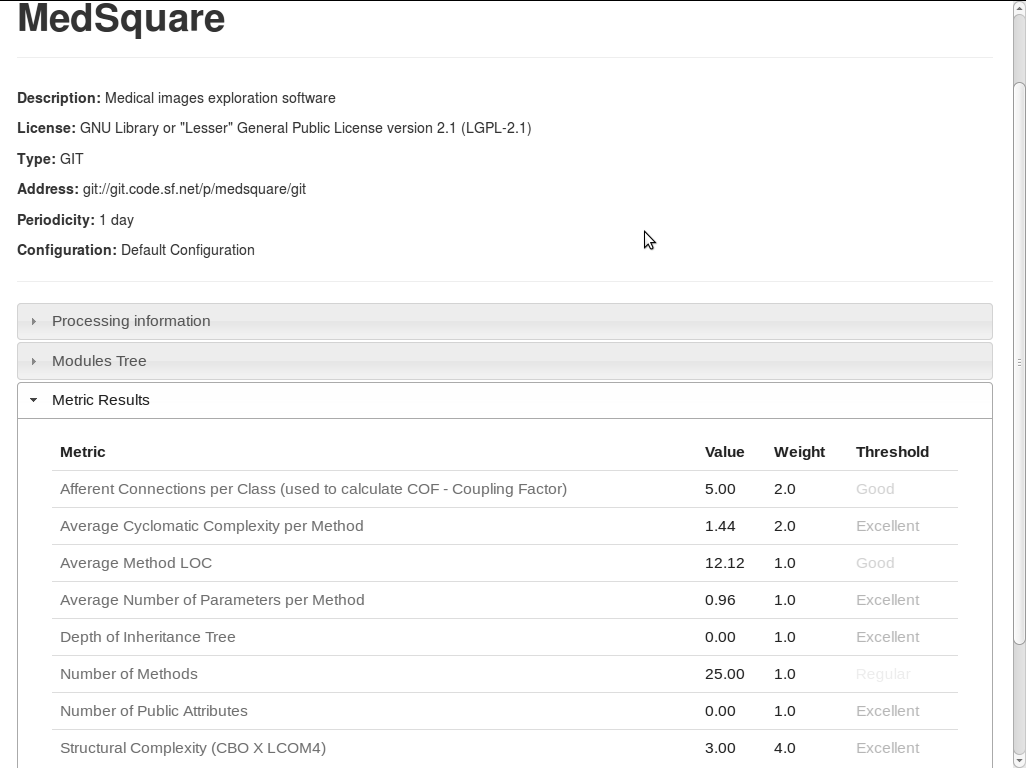
\includegraphics[width=\textwidth]{images/new-repository-results.png}
    \caption{Tela de visualização dos resultados do processamento do repositório.}
    \label{fig:results}
  \end{figure}

\section{Conclusão}
O Mezuro surge como uma potencial resposta para a falta de monitoramento e padronização de código-fonte e a necessidade de avaliação do mesmo, considerando que é um \textit{software} livre, altamente customizável, com suporte para muitas linguagens computacionais, interface amigável, que fornece histórico de processamentos e também com uma arquitetura planejada para incorporar novas funcionalidades.

\bibliographystyle{splncs03}
\bibliography{mezuro}
\end{document}
